\section{Cryptographie}
\framewithtitle{Cryptographie}

\begin{frame}{Sommaire}
  \setcounter{tocdepth}{2}
  \tableofcontents[currentsection, hideothersubsections]
\end{frame}

\begin{frame}{Objectifs de ce module}
  Comprendre les opérations de base de la cryptographie
  \begin{enumerate}
    \item Hachage
    \item Chiffrement symétrique/asymétrique
    \item Signature digitale
  \end{enumerate}
\end{frame}

\begin{frame}{Notations}
  \begin{tiny}
    \textit{Je suis désolé, il faut faire un tout petit peu de maths...}
  \end{tiny}

  Dans la suite, je vais noter :

  \begin{itemize}
    \item $\mathbb{B} = \{0,1\}^\mathbb{N}$ l'ensemble des mots binaires
    \item $\mathbb{B}_{n \in \mathbb{N}} = \{0,1\}^n$ l'ensemble des mots binaires de taille $n$
  \end{itemize}

  Exemples :

  \begin{itemize}
    \item $B_3 = \{000, 001, 010, 011, 100, 101, 110, 111\}$
    \item $010010$ est un mot binaire de 6 bits, il est donc membre de $\mathbb{B}_6$
  \end{itemize}
\end{frame}

\begin{frame}{Qu'est-ce que la cryptographie ?}
  \begin{columns}
    \begin{column}{0.65\textwidth}
      TL;DR = utiliser les mathématiques au service de la sécurité de l'information

      Exemples historiques :
      \begin{itemize}
        \item Chiffrement de César : décalage de lettre de 1 à 25
        \item Chiffrement de Vigenère : sustitions de lettres à partir d'une clé secrète
        \item Chiffrement affine : subsutition de lettre à l'aide d'une équation affine
        \item Enigma (seconde guerre modiale) : machine de chiffrement allemande
      \end{itemize}
    \end{column}

    \begin{column}{0.3\textwidth}
      \begin{figure}
  \resizebox{\textwidth}{!}{
    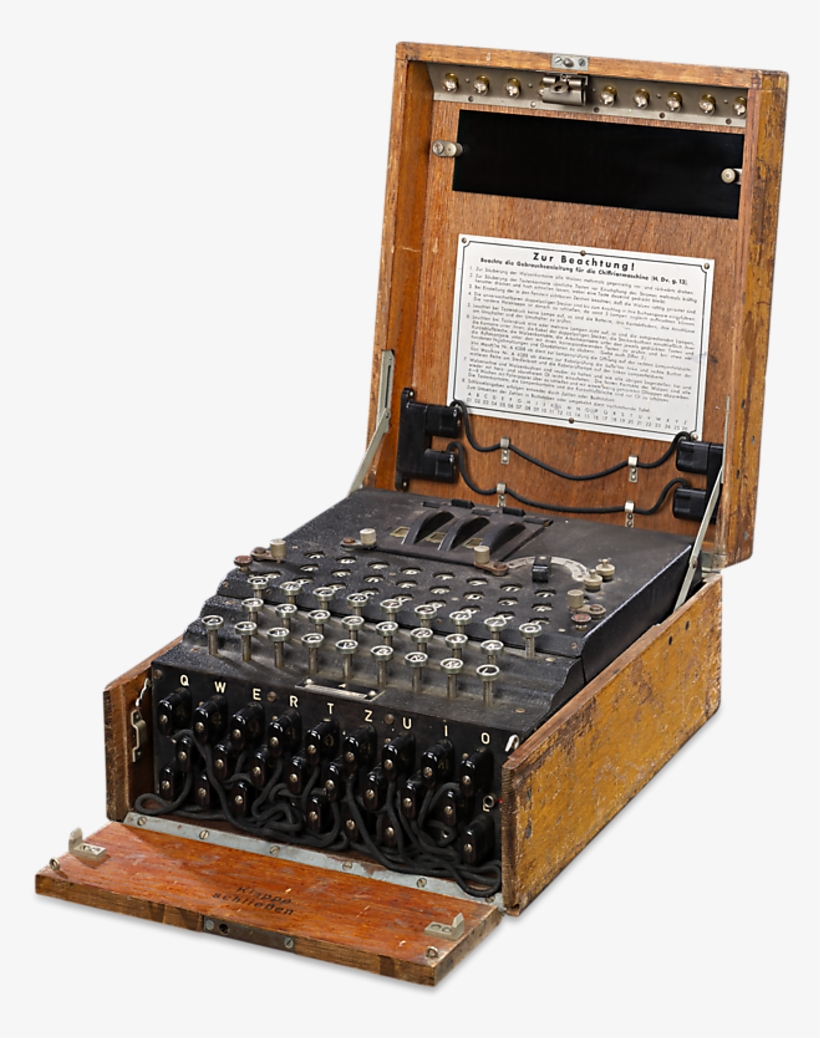
\includegraphics{img/enigma.png}
  }

  \caption{Machine Enigma}
  \label{fig:enigma}
\end{figure}
    \end{column}
  \end{columns}
\end{frame}

\subsection*{Somme de contrôle}

\begin{frame}{Somme de contrôle : définition}
  \begin{block}{Définition : somme de contrôle}
    Une somme de contrôle est une petite quantité de données additionnelle qui est calculée à partir d'un ensemble plus large de données. Elle est utilisée pour vérifier l'intégrité des données et détecter les erreurs ou les altérations éventuelles.
  \end{block}

  Exemples :

  \begin{itemize}
    \item Numéro de sécurité sociale
    \item Numéro de carte bancaire
    \item IBAN
    \item Mémoire ECC (Error Correcting Code)
  \end{itemize}
\end{frame}

\begin{frame}[fragile]{Somme de contrôle : exemple du numéro de sécurité sociale}
  Les deux derniers chiffre du numéro de sécurité sociale ne contiennent aucune information mais ils sont utilisés comme somme contrôle, pour limiter les risques de faute d'erreur.

  La formule permettant de calculer la clé est la suivante :

  $$
    \textrm{clé} = 97 - NIR \bmod 97
  $$

  $$
    \underbrace{2 69 05 49 588 157}_{\textrm{numéro NIR}}\underbrace{80}_{\textrm{clé}}
  $$

  \begin{minted}{text}
      >>> 97 - 2690549588157 % 97
      80
    \end{minted}
\end{frame}
\subsection{Hachage}

\begin{frame}{Fonction de hachage : définition}
  \begin{columns}
    \begin{column}{0.7\textwidth}
      Comment appliquer cette logique à de l'information binaire ?
      On cherche une somme de contrôle universelle capable de fonctionner sur tout $\mathbb{B}$.

      $\Rightarrow$ on les appelle fonction de hachage

      \begin{block}{Définition : fonction de hachage}
        Une fonction de hachage permet de générer un \textquote{hash} de n'importe quel mot binaire.
      \end{block}

      \begin{block}{Définition : hash}
        Un hash est un mot binaire de taille fixe, dont la taille est spécifique à la fonction de hachahe utilisé.
      \end{block}
    \end{column}
    \begin{column}{0.2\textwidth}
      \resizebox{\textwidth}{!}{
        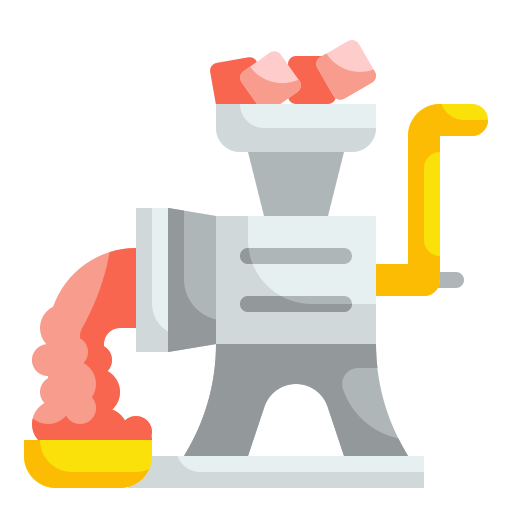
\includegraphics{img/meat-grinder.png}
      }
    \end{column}
  \end{columns}
\end{frame}

\begin{frame}[fragile]{Fonction de hachage : exemples}
  \begin{figure}
  \begin{minted}{text}
    >>> import hashlib
    >>> hashlib.md5(b"Mathieu").hexdigest()
    '206299fa740a4327a61b67b6be5c8373'
  \end{minted}

  \caption{Calcul d'un MD5 en ligne de commande en Python}
  \label{code:md5-hash-cli}
\end{figure}
  \begin{figure}
  \begin{minted}{text}
    >>> import hashlib
    >>> hashlib.sha256(b"Mathieu").hexdigest()
    'f5e088d29801ebb822251d7751bc4b8ff28c50132d8b0a95614b5f048a1d01b6'
  \end{minted}

  \caption{Calcul d'un SHA-256 en ligne de commande en Python}
  \label{code:sha256-hash-cli}
\end{figure}
\end{frame}

\begin{frame}{Caractéristiques d'une fonction de hachage}
  \begin{block}{Uniformité}
    Une bonne fonction de hachage doit répartir uniformément les valeurs d'entrée sur l'ensemble des valeurs de hachage possibles. Cela signifie que des entrées différentes doivent avoir une probabilité égale de générer des valeurs de hachage différentes.
  \end{block}

  \begin{block}{Déterminisme}
    Pour une même valeur d'entrée, la fonction de hachage doit toujours générer la même valeur de hachage. Cela permet d'obtenir des résultats cohérents et reproductibles.


  \end{block}
\end{frame}

\begin{frame}{Caractéristiques d'une fonction de hachage}
  \begin{block}{Résistance aux collisions}
    Une fonction de hachage $h$ de taille $n$ entraîne obligatoirement des collisions car la taille de $\mathbb{B}$ est infinie alors que $\mathbb{B}_n$ n'est \textquote{que} de $2^n$.
    Une collision existe quand deux mots binaires $a$ et $b$ engendrent le même hash, c'est-à-dire :

    $$h(a) = h(b)$$

    $\Rightarrow$ une \textquote{bonne} fonction de hachage ne possède pas de hash connu.

    \begin{small}
      \textit{Note : Les algorithmes md4, md5 et sha1 ne sont à jour plus considérés comme sûrs.}
    \end{small}
  \end{block}
\end{frame}

\begin{frame}{Caractéristiques d'une fonction de hachage}
  \begin{block}{Sensibilité aux changements}
    Une petite modification dans l'entrée doit entraîner un changement significatif dans la valeur de hachage.
    Cela garantit que des entrées similaires génèrent des valeurs de hachage différentes.
  \end{block}

  \begin{figure}
  \resizebox{\columnwidth}{!}{%
    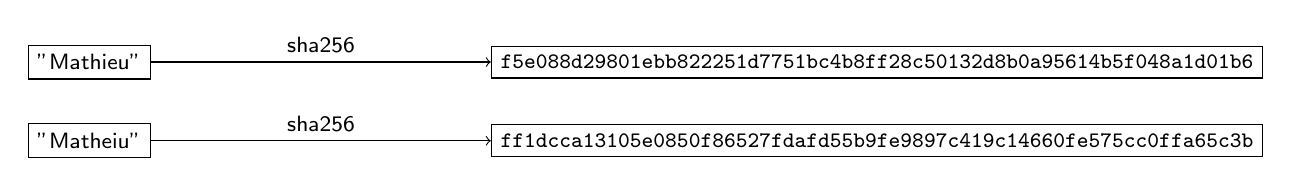
\begin{tikzpicture}[font=\sffamily\footnotesize,
        Input/.style={shape=rectangle,draw},
        Output/.style={shape=rectangle,draw}
      ]

      \node[Input] (I_1) at (0,0) {"Mathieu"};
      \node[Output] (O_1) at (10,0) {\texttt{f5e088d29801ebb822251d7751bc4b8ff28c50132d8b0a95614b5f048a1d01b6}};
      \node[Input] (I_2) at (0,-1) {"Matheiu"};
      \node[Output] (O_2) at (10,-1) {\texttt{ff1dcca13105e0850f86527fdafd55b9fe9897c419c14660fe575cc0ffa65c3b}};

      \draw[->] (I_1) -- (O_1) node[midway,above,sloped]{sha256};
      \draw[->] (I_2) -- (O_2) node[midway,above,sloped]{sha256};
    \end{tikzpicture}%
  }

  \caption{Sensibilité aux changements de la fonction SHA-256}
  \label{fig:sha256-hash-examples}
\end{figure}
\end{frame}

\begin{frame}{Caractéristiques d'une fonction de hachage}
  \begin{block}{Efficacité}
    Une bonne fonction de hachage doit être rapide à calculer pour des données de toutes tailles.
    Les performances de la fonction de hachage sont essentielles, car elle est souvent utilisée dans des applications nécessitant des opérations rapides sur de grandes quantités de données.

    \vspace*{1em}

    Ces performanaces sont tellement cruciales que certains algorithmes de hachage sont directement implémentés en tant qu'instructions dans les processeurs.
    Par exemple, les algorithmes SHA-1 et SHA-256 sont \textbf{matériellement} présents dans tous les processeurs Intel depuis 2013.
  \end{block}
\end{frame}

\begin{frame}{Caractéristiques d'une fonction de hachage}
  \begin{block}{Le plus important : résistance aux attaques}
    Une fonction de hachage sécurisée doit être résistante à différentes attaques, telles que :

    \begin{itemize}
      \item les attaques de collisions
      \item les attaques de préimage
      \item les attaques par force brute
    \end{itemize}

    Elle doit être suffisamment robuste pour empêcher un adversaire de trouver des \textbf{collisions intentionnelles} ou de retrouver \textbf{l'entrée d'origine à partir de la valeur de hachage}.
  \end{block}
\end{frame}

\begin{frame}{Fonction de hachage : résumé}
  \begin{itemize}
    \item Une fonction de hachage prend n'importe quel mot binaire entrée et retourne un mot binaire de taille fixe
    \item Une bonne fonction de hachage possède les caractéristiques suivantes :
          \begin{itemize}
            \item Uniformité
            \item Déterminisme (= pas de hasard)
            \item Résistance aux collisions
            \item Sensibilité aux changements
            \item Efficacité
            \item \textbf{Résistance aux attaque bruteforce / reverse}
          \end{itemize}
  \end{itemize}
\end{frame}

\begin{frame}{Fonction de hachage : exercices}
  \begin{block}{Exercice 1 : se familiariser avec les fonctions de hachage}
    En CLI, calculez le hash de votre prénom / animal / n'importe quoi.
    Vous pouvez utiliser des bibliothèques ou des outils en ligne pour effectuer ce calcul.
    Comparez ensuite la valeur de hachage obtenue avec celle d'autres chaînes de caractères.
    Observez comment une légère modification de la chaîne d'entrée entraîne un changement significatif dans la valeur de hachage.
  \end{block}

  \begin{block}{Exercice 2 : calcul du hash d'un fichier}
    Calculez le hash du whitepaper du bitcoin, accessible sur \url{https://bitcoin.org/bitcoin.pdf}.
    Comparez sa valeur avec les autres.
  \end{block}
\end{frame}
\subsection{Chiffrement symétrique}

\begin{frame}{Chiffrement : définition}
  \begin{block}{Définition : chiffrement}
    Le chiffrement est une technique permettant à deux parties d'échanger de manière sécurisée.
    Il existe deux grands types de chiffrements, dits symétrique et asymétrique.

    Les principales caractéristiques du chiffrement sont :

    \begin{itemize}
      \item Confidentialité : protéger contre l'accès non autorisé, seules les personnes ayant la clé puissent déchiffrer et lire le message.
      \item Intégrité : détecter toute modification ou altération des données chiffrées. Si les données chiffrées sont altérées, le déchiffrement donnera un résultat incorrect ou une erreur.
      \item Efficacité : traiter rapidement les données, en particulier lorsqu'il s'agit de volumes importants.
      \item Sécurité : être résistants aux attaques cryptographiques, telles que les attaques par force brute, les attaques de collision, différentielles\dots
    \end{itemize}
  \end{block}
\end{frame}

\begin{frame}{Modèle de canal de communication}
  \begin{figure}
  \resizebox{\columnwidth}{!}{%
    \begin{tikzpicture}
      % Actors
      \node[label=Alice] (alice) at (0,0) {
\includegraphics[height=4cm]{img/alice.png}};
      \node[label=Bob] (bob) at (24,0) {
\includegraphics[height=4cm]{img/bob.png}};
      \node[label=Eve] (eve) at (12,-4) {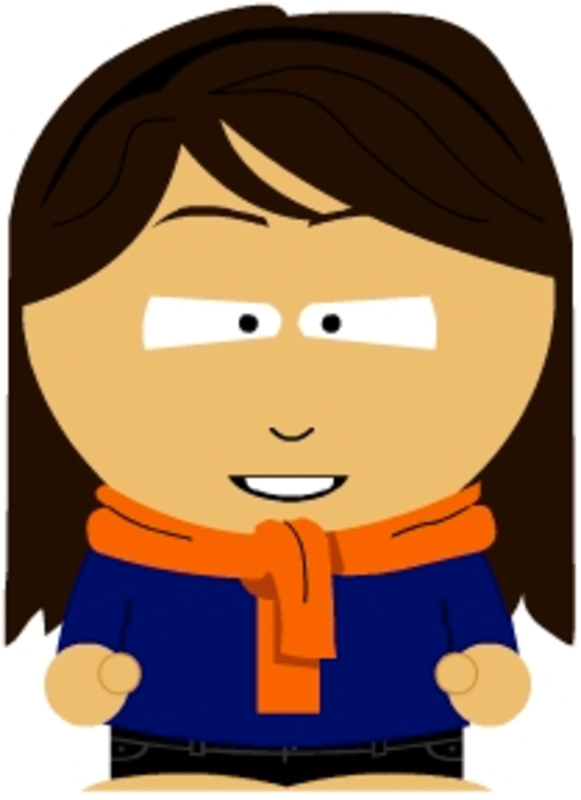
\includegraphics[height=4cm]{img/eve.png}};

      % Canal
      \draw (4,0) ellipse (0.35 and 0.5);
      \draw (20,-0.5) arc (-90:90:0.5);
      \draw (4,0.5) -- ++(16,0);
      \draw (4,-0.5) -- ++(16,0);
      \node (label) at (12, 1) {Canal de communication non sécurisé};

      \draw[->] (eve.west) -- ++(-1.5,0) -- node[left] {Écoute} ++(0,3.5);
      \draw[->] (eve.east) -- ++(1.5,0) --  node[right] {Modifie} ++(0,3.5);

    \end{tikzpicture}%
  }

  \caption{Modèle de canal de communication non sécurisé}
\end{figure}
\end{frame}

\begin{frame}{Chiffrement symétrique}
  \begin{block}{Définition : chiffrement symétrique}
    Le chiffrement symétrique est une technique de chiffrement où \textbf{une seule et même clé} est utilisée à la fois pour le \textbf{chiffrement et le déchiffrement} des données.
    Cela signifie que l'émetteur et le destinataire du message doivent partager la même clé secrète pour pouvoir communiquer de manière sécurisée.

    \vspace{1em}

    Exemples d'algorithmes de chiffrement symétriques :

    \begin{itemize}
      \item AES
      \item DES (obslète) et triple DES
    \end{itemize}
  \end{block}
\end{frame}

\begin{frame}{Chiffrement symétrique : modèle}
  \begin{figure}
  \resizebox{\columnwidth}{!}{%
    \begin{tikzpicture}
      % Actors
      \node[label=Alice + clé $K$] (alice) at (0,0) {
\includegraphics[height=4cm]{img/alice.png}};
      \node[label=Bob + clé $K$] (bob) at (24,0) {
\includegraphics[height=4cm]{img/bob.png}};
      \node[label=Eve sans clé] (eve) at (12,-4) {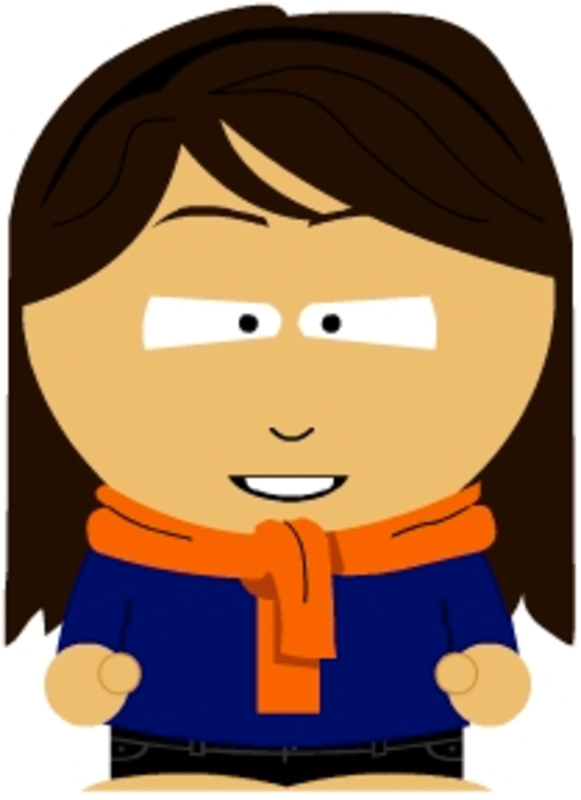
\includegraphics[height=4cm]{img/eve.png}};

      \node[draw] (alice_clear) at (3,0) {Message};
      \node[draw] (cipher) at (12,0) {\#\&*YU*F};
      \node[draw] (bob_clear) at (21,0) {Message};

      \draw[->] (alice_clear.east) -- (cipher) node[near start,above,sloped]{Chiffre avec $K$};
      \draw[->] (cipher.east) -- (bob_clear) node[near end,above,sloped]{Déchiffre avec $K$};

      % Canal
      \draw (8,0) ellipse (0.35 and 0.5);
      \draw (16,-0.5) arc (-90:90:0.5);
      \draw (8,0.5) -- ++(8,0);
      \draw (8,-0.5) -- ++(8,0);
      \node (label) at (12, 1) {Canal de communication non sécurisé};

      \draw[->] (eve.west) -- ++(-1.5,0) -- node[left] {Écoute} ++(0,3.5);
      \draw[->] (eve.east) -- ++(1.5,0) --  node[right] {Modifie} ++(0,3.5);
    \end{tikzpicture}%
  }

  \caption{Chiffrement symétrique avec une clé $K$}
\end{figure}
\end{frame}

\begin{frame}{Chiffrement symétrique : exercice}
  \begin{block}{Exercice : échange d'information sur canal public}
    \begin{enumerate}
      \item Aller sur \url{https://www.devglan.com/online-tools/aes-encryption-decryption}
      \item Choisir une clé de 32 caractères hexadécimaux (par ex: \texttt{770A8A65DA156D24EE2A093277530142}).
      \item Partager la clé avec un ami.
      \item Chiffrer un message et le publier sur un canal public.
      \item Vérifier que l'ami est capable de déchiffrer le message et personne d'autre.
    \end{enumerate}
  \end{block}
\end{frame}

\begin{frame}{Chiffrement symétrique : résumé}
  \begin{itemize}
    \item Le chiffrement symétrique permet d'échanger des messages secrets.
    \item Une seule clé pour chiffrer et déchiffrer $\Rightarrow$ l'émetteur et le destinataire doivent connaître la clé.
    \item AES est l'algorithme le plus utilisé.
  \end{itemize}

  Problème : comment partager la clé de manière sécurisée ?
\end{frame}

\begin{frame}{Modes de chiffrement}
  \begin{columns}
    \begin{column}{0.6\textwidth}
      \begin{itemize}
        \item ECB (Electronic CodeBook)
          \begin{itemize}
            \item Le plus simple mais le moins sécurisé
            \item Motifs visibles dans les données chiffrées
          \end{itemize}
        \item CBC (Cipher Block Chaining)
          \begin{itemize}
            \item Utilise un vecteur d'initialisation (IV)
            \item Chaque bloc dépend du précédent
          \end{itemize}
        \item CTR (Counter)
          \begin{itemize}
            \item Transforme le chiffrement par bloc en flux
            \item Parallélisable
          \end{itemize}
        \item GCM (Galois/Counter Mode)
          \begin{itemize}
            \item Authentification intégrée
            \item Recommandé pour TLS
          \end{itemize}
      \end{itemize}
    \end{column}
    \begin{column}{0.4\textwidth}
      \begin{center}
        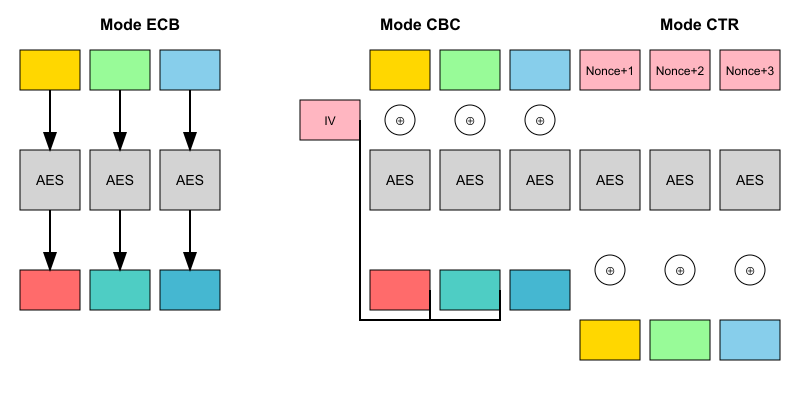
\includegraphics[width=\textwidth]{img/encryption-modes.png}
      \end{center}
    \end{column}
  \end{columns}
\end{frame}

\begin{frame}[fragile]{Exemple pratique avec Node.js}
  \begin{minted}[fontsize=\scriptsize]{javascript}
    const crypto = require('crypto');

    // Génération de la clé et du vecteur d'initialisation
    const key = crypto.randomBytes(32); // 256 bits pour AES-256
    const iv = crypto.randomBytes(16);  // 128 bits pour AES

    // Chiffrement
    function encrypt(text) {
      const cipher = crypto.createCipheriv(
        'aes-256-cbc', key, iv
      );
      let encrypted = cipher.update(text, 'utf8', 'hex');
      encrypted += cipher.final('hex');
      return encrypted;
    }

    // Déchiffrement
    function decrypt(encrypted) {
      const decipher = crypto.createDecipheriv(
        'aes-256-cbc', key, iv
      );
      let decrypted = decipher.update(encrypted, 'hex', 'utf8');
      decrypted += decipher.final('utf8');
      return decrypted;
    }

    const message = "Message secret";
    const encrypted = encrypt(message);
    console.log("Chiffré:", encrypted);
    console.log("Déchiffré:", decrypt(encrypted));
  \end{minted}

  \begin{itemize}
    \item Utilise AES-256 en mode CBC
    \item Gestion explicite de la clé et de l'IV
    \item Format hexadécimal pour le texte chiffré
  \end{itemize}
\end{frame}

\begin{frame}{Applications courantes}
  \begin{itemize}
    \item Chiffrement de disque
      \begin{itemize}
        \item BitLocker (Windows)
        \item FileVault (macOS)
        \item LUKS (Linux)
      \end{itemize}
    \item Communications sécurisées
      \begin{itemize}
        \item WiFi (WPA3)
        \item VPN
        \item Session TLS
      \end{itemize}
    \item Stockage cloud
      \begin{itemize}
        \item Chiffrement côté client
        \item Chiffrement au repos
      \end{itemize}
  \end{itemize}
\end{frame}

\begin{frame}{Performance et sécurité}
  \begin{columns}
    \begin{column}{0.5\textwidth}
      Tailles de clé courantes :
      \begin{itemize}
        \item AES-128 : 128 bits
        \item AES-192 : 192 bits
        \item AES-256 : 256 bits
      \end{itemize}

      Performances :
      \begin{itemize}
        \item Instructions AES-NI
        \item \textasciitilde 1 Go/s sur CPU moderne
        \item Adapté au chiffrement temps réel
      \end{itemize}
    \end{column}

    \begin{column}{0.5\textwidth}
      Bonnes pratiques :
      \begin{itemize}
        \item Rotation régulière des clés
        \item Stockage sécurisé des clés
        \item Utilisation de sel (IV)
        \item Mode authentifié (GCM)
      \end{itemize}
    \end{column}
  \end{columns}
\end{frame}
\subsection{Chiffrement asymétrique}

\begin{frame}{Chiffrement asymétrique}
  \begin{block}{Définition : chiffrement asymétrique}
    Le chiffrement asymétrique, également connu sous le nom de cryptographie à clé publique, est une technique de chiffrement qui utilise une paire de clés distinctes pour le processus de chiffrement et de déchiffrement des données.

    Cette paire de clés est composée d'une clé publique et d'une clé privée. Elles sont liées mathématiquement. On peut alors chiffre un message avec la clé publique et déchiffrer le message avec la clé privée.
  \end{block}

  Cela permet de recevoir des messages de manière sécurisée sans échange de clé au préalable.

  \begin{enumerate}
    \item Alice publie sa clé publique (par exemple sur son profil GitHub).
    \item Bob va la contacter et lui envoie un message chiffré avec la clé publique d'Alice
    \item Alice déchiffre le message avec sa clé privée.
  \end{enumerate}
\end{frame}

\begin{frame}[fragile]{Chiffrement asymétrique : exemple}
  On considère un algorithme de chiffrement asymétrique générique :

  \begin{minted}{python}
    def cipher(data: str, key: str) -> str:
    def decipher(data: str, key: str) -> str:

    message = "Hello world"
    private_key, public_key = generateKeys()

    result = cipher(message, public_key)  # "&*#&*#QQ#)"
    clear = decipher(result, private_key) # "Hello world"
  \end{minted}
\end{frame}

\begin{frame}{Chiffrement asymétrique : communication sécurisée}
  \begin{figure}
  \resizebox{\columnwidth}{!}{%
    \begin{tikzpicture}
      % Actors
      \node[label=Alice + clé $P_k$] (alice) at (0,0) {
\includegraphics[height=4cm]{img/alice.png}};
      \node[label=Bob + clé $P_k$ et $S_k$] (bob) at (24,0) {
\includegraphics[height=4cm]{img/bob.png}};
      \node[label=Eve + clé $P_k$] (eve) at (12,-4) {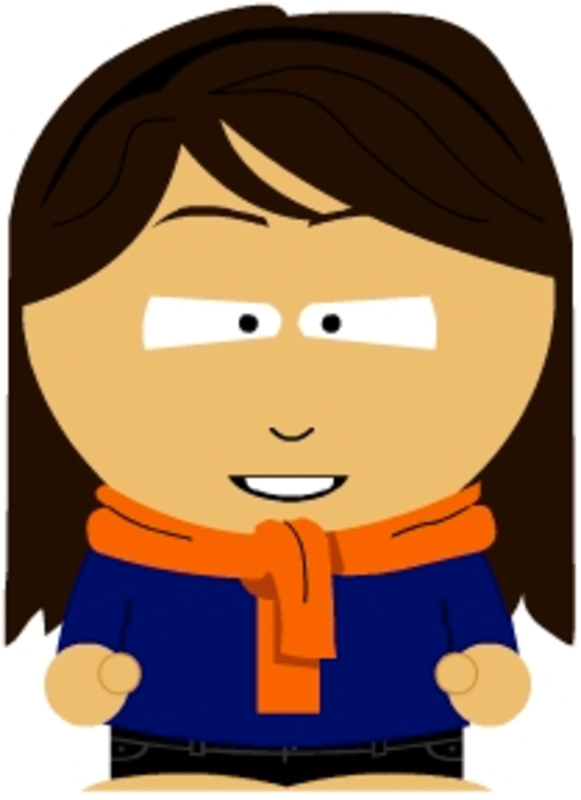
\includegraphics[height=4cm]{img/eve.png}};

      \node[draw] (alice_clear) at (3,0) {Message};
      \node[draw] (cipher) at (12,0) {\#\&*YU*F};
      \node[draw] (bob_clear) at (21,0) {Message};

      \draw[->] (alice_clear.east) -- (cipher) node[near start,above,sloped]{Chiffre avec $P_k$};
      \draw[->] (cipher.east) -- (bob_clear) node[near end,above,sloped]{Déchiffre avec $S_k$};

      % Canal
      \draw (8,0) ellipse (0.35 and 0.5);
      \draw (16,-0.5) arc (-90:90:0.5);
      \draw (8,0.5) -- ++(8,0);
      \draw (8,-0.5) -- ++(8,0);
      \node (label) at (12, 1) {Canal de communication non sécurisé};

      \draw[->] (eve.west) -- ++(-1.5,0) -- node[left] {Écoute} ++(0,3.5);
      \draw[->] (eve.east) -- ++(1.5,0) --  node[right] {Modifie} ++(0,3.5);
    \end{tikzpicture}%
  }

  \caption{Chiffrement asymétrique avec une clé $(P_k,S_k)$}
\end{figure}
\end{frame}

\begin{frame}{Combinaison asymétrique/symétrique}
  L'utilisation des deux techniques de chiffrement permet de communiquer de manière sécuriser sans avoir à faire un échange de clé au préalable.

  \begin{enumerate}
    \item Bob génère son couple de clés $(P_k,S_k)$ et publie sa clé publique $P_k$
    \item Alice veut communiquer avec Bob. Elle génère une clé de chiffrement symétrique $K$.
    \item Alice chiffre $K$ avec la clé publique de Bob $P_k$ et envoie le message chiffré à Bob.
    \item Bob déchiffre le message d'Alice avec sa clé privée $S_k$ et se retrouve donc en possession de la clé $K$.
    \item Par la suite, Alice et Bob utilise la clé $K$ et un algorithme de chiffrement symétrique pour communiquer.
  \end{enumerate}
\end{frame}
\subsection{Signature numérique}

\begin{frame}{Signature numérique : définition}
  \begin{block}{Définition : signature numérique}
    Une signature numérique est un mécanisme cryptographique utilisé pour authentifier l'intégrité et l'origine d'un message, d'un document électronique ou d'un ensemble de données.

    Elle sert à garantir qu'un document n'a pas été altéré depuis sa signature et qu'il provient bien de l'expéditeur prétendu.

    La signature numérique repose sur des algorithmes de cryptographie asymétrique, qui utilisent une paire de clés : une clé privée et une clé publique.

    L'expéditeur utilise sa clé privée pour générer une signature numérique unique basée sur le contenu du document.
    Cette signature est ensuite jointe au document, qui peut être transmis à d'autres parties.
  \end{block}
\end{frame}

\begin{frame}{Signature numérique : exemple}
  \begin{enumerate}
    \item Alice génère sa paire de clé publique/privée $(P_k, S_k)$
    \item Alice publie sa clé publique $P_k$
    \item Alice veut signer le message \textquote{Alice donne 1 BTC à Bob}
          \begin{enumerate}
            \item Alice calcule le hash de \textquote{Alice donne 1 BTC à Bob}
            \item Alice chiffre le hash avec sa clé privée et diffuse le message+le hash signé
          \end{enumerate}
    \item Tout individu peut maintenant vérifier que le message qu'Alice a chiffré est bien le hash du message qu'elle a publié
    \item[$\Rightarrow$] Alice a \textbf{signé} le message \textquote{Alice donne 1 BTC à Bob}
  \end{enumerate}
\end{frame}

\begin{frame}{Algorithmes de signature numérique}
  \begin{itemize}
    \item RSA-PSS
      \begin{itemize}
        \item Version signature de RSA
        \item Padding probabiliste
        \item Largement utilisé
      \end{itemize}
    \item ECDSA
      \begin{itemize}
        \item Basé sur les courbes elliptiques
        \item Utilisé dans Bitcoin
        \item Signatures plus courtes que RSA
      \end{itemize}
    \item EdDSA
      \begin{itemize}
        \item Variante d'ECDSA avec Curve25519
        \item Plus rapide et plus sûr
        \item Utilisé dans SSH et Signal
      \end{itemize}
  \end{itemize}
\end{frame}

\begin{frame}[fragile]{Exemple pratique avec Node.js}
  \begin{columns}
    \begin{column}{0.48\textwidth}
      \begin{minted}[fontsize=\scriptsize]{javascript}
const crypto = require('crypto');

// Génération des clés
const { privateKey, publicKey } = 
  crypto.generateKeyPairSync('ec', {
    namedCurve: 'secp256k1',
    publicKeyEncoding: {
      type: 'spki',
      format: 'pem'
    },
    privateKeyEncoding: {
      type: 'pkcs8',
      format: 'pem'
    }
  });
      \end{minted}
    \end{column}

    \begin{column}{0.48\textwidth}
      \begin{minted}[fontsize=\scriptsize]{javascript}
// Message à signer
const message = "Transaction: Alice -> Bob 1 BTC";

// Signature
const signer = crypto.createSign('SHA256');
signer.update(message);
const signature = signer.sign(privateKey);

// Vérification
const verifier = crypto.createVerify('SHA256');
verifier.update(message);
const isValid = verifier.verify(
  publicKey, 
  signature
);
console.log(isValid ? "Valide!" : "Invalide!");
      \end{minted}
    \end{column}
  \end{columns}
\end{frame}

\begin{frame}{Applications des signatures numériques}
  \begin{columns}
    \begin{column}{0.5\textwidth}
      Documents électroniques :
      \begin{itemize}
        \item Contrats numériques
        \item Factures électroniques
        \item Documents administratifs
      \end{itemize}

      Code et logiciels :
      \begin{itemize}
        \item Signature de code
        \item Mises à jour système
        \item Paquets logiciels
      \end{itemize}
    \end{column}

    \begin{column}{0.5\textwidth}
      Blockchain :
      \begin{itemize}
        \item Transactions
        \item Smart contracts
        \item Gouvernance DAO
      \end{itemize}

      Communication :
      \begin{itemize}
        \item Email (S/MIME, PGP)
        \item Messages instantanés
        \item Certificats TLS
      \end{itemize}
    \end{column}
  \end{columns}
\end{frame}

\begin{frame}{Aspects juridiques}
  \begin{block}{Cadre légal}
    En Europe, le règlement eIDAS définit trois niveaux de signature électronique :
    \begin{itemize}
      \item Simple : basique, peu de valeur légale
      \item Avancée : cryptographiquement sûre
      \item Qualifiée : maximum de valeur légale
    \end{itemize}
  \end{block}

  Exigences pour une signature qualifiée :
  \begin{itemize}
    \item Certificat qualifié
    \item Dispositif sécurisé de création
    \item Horodatage qualifié
    \item Conservation à long terme
  \end{itemize}
\end{frame}

\begin{frame}{Bonnes pratiques}
  \begin{itemize}
    \item Sécurité des clés privées
      \begin{itemize}
        \item Stockage sécurisé (HSM)
        \item Sauvegarde et récupération
        \item Rotation périodique
      \end{itemize}
    \item Vérification
      \begin{itemize}
        \item Validation du certificat
        \item Vérification de révocation
        \item Horodatage
      \end{itemize}
    \item Format et standards
      \begin{itemize}
        \item PAdES pour PDF
        \item XAdES pour XML
        \item CAdES pour données binaires
      \end{itemize}
  \end{itemize}
\end{frame}